\documentclass[10pt,a4paper]{article}
\usepackage[margin=1.8cm]{geometry}
\usepackage[T1]{fontenc}
\usepackage{lmodern}
\usepackage{graphicx,booktabs,amsmath,array,xcolor}
\usepackage[hidelinks]{hyperref}
\setlength{\parindent}{0pt}
\setlength{\parskip}{5pt}
\title{Centralized and Federated Skin-Lesion Classification\\\large Stage 1: Baseline Development and Minimal Federated Setup}
\author{Alfred Pietraru \and Stefan Dascalu}
\date{11 November 2026}
\begin{document}
\maketitle
\vspace{-1.5em}
\begin{abstract}
We investigate eight-class ISIC 2019 classification with a pretrained ResNet-18 and Flower. Centralized experiments compare optimization, focal loss, and resampling, reaching test macro-F1 near 0.52. Four-client non-IID FedAvg reaches weighted client validation macro-F1 of 0.373 after ten rounds. Different data fractions, batch sizes, and metric aggregation prevent isolating the cost of federation; minority-class and client disparities motivate Stage 2.
\end{abstract}

\section{Motivation and research questions}
Medical image collections can be distributed across institutions with different class frequencies. This project examines whether a practical classifier can be trained centrally and through model aggregation while keeping image records within their assigned client partitions. The experiment uses simulated hospitals on one machine; it does not establish privacy protection or clinical effectiveness.

The Stage 1 questions are: \textbf{RQ1}, how do optimizer settings, focal loss, and resampling affect centralized validation and test performance under severe class imbalance? \textbf{RQ2}, can a four-client non-IID FedAvg setup learn a useful global classifier, and how heterogeneous are client outcomes? \textbf{RQ3}, which evaluation gaps must be resolved before a controlled centralized--federated comparison and a trustworthiness study?

\section{Related work and literature comparison}
Ahmad et al.~\cite{ahmad2026} benchmark imbalance mitigation with pretrained CNNs, Adam at $10^{-4}$, and geometric augmentation. Gayatri and Aarthy~\cite{gayatri2024} study augmentation and focal loss with ResNet-50. Cino et al.~\cite{cino2025} study test-time augmentation and CNN explainability, informing our transfer-learning and augmentation approach. These papers influenced optimizer exploration, transformations, and imbalance handling. AdamW, our crop pipeline, and 90-degree rotations are project adaptations. Cino et al.'s Grad-CAM analysis also motivates future interpretability work; test-time augmentation and explanation maps are not evaluated here. Our split and checkpoint protocol differ from the papers, so published scores are not directly compared.

\section{Dataset and preprocessing}
The local ground-truth/EDA archive contains 25,331 dermoscopic images over eight labels: MEL (melanoma), NV (melanocytic nevus), BCC (basal cell carcinoma), AK (actinic keratosis), BKL (benign keratosis), DF (dermatofibroma), VASC (vascular lesion), and SCC (squamous cell carcinoma). NV accounts for 12,875 images (50.83\%), whereas DF has 239 (0.94\%): a 53.9:1 imbalance. Accuracy alone is therefore insufficient.

Images are decoded as RGB. Samples with a recorded lesion identifier are grouped before stratified splitting; groups use their majority label, with deterministic tie-breaking. Missing lesion identifiers fall back to image identifiers, so lesion-based grouping cannot guarantee patient independence. Fractions apply to groups and therefore only approximately to image counts.

\textbf{Reducing training imbalance.} After splitting, random undersampling removes 60\% of NV training entries (10,318 to 4,128). Random oversampling duplicates AK, DF, VASC, and SCC entries once; other classes are unchanged. This reduces NV's training share from 51.0\% to 26.5\% and the largest/smallest class ratio from 52.1:1 to 10.4:1. It is partial rebalancing, not equalization. The resulting 15,605 entries include 1,559 duplicates of existing minority images; no new independent lesions are created. Stochastic augmentation can produce different views of repeated images. Validation and test data are not resampled.

\newpage
\section{Centralized baseline and experimental protocol}
\textbf{Architecture.} The implementation fine-tunes an ImageNet-initialized ResNet-18, replacing its final fully connected layer with an eight-output classifier. All model parameters are passed to the optimizer; the backbone is not frozen. Raw logits are used by the loss and softmax probabilities by evaluation metrics.

\textbf{Preprocessing.} Archived run configurations resize images to $512\times512$. Training then takes a central $288\times288$ region and a random $224\times224$ crop, applies independent flips on both spatial axes with probability 0.5, and random 90-degree rotations with probability 0.5. Validation/test use a central $224\times224$ crop after resizing. Intensities are scaled from $[0,255]$ to $[0,1]$ and normalized by ImageNet channel means $(0.485,0.456,0.406)$ and standard deviations $(0.229,0.224,0.225)$. Central cropping may remove useful lesion context; no cropping ablation establishes an advantage.

\textbf{Data and optimization.} Centralized runs use seed 42 and group fractions 0.8/0.1/0.1, producing 20,236 training, 2,667 validation, and 2,428 test images before resampling. Batch size is 128, with eight loader workers in the archived configurations. The fine-tuning runs use AdamW with learning rate $10^{-4}$ and weight decay $10^{-3}$. ReduceLROnPlateau uses validation loss, factor 0.5, and patience 3. The configured maximum is 100 epochs; early stopping uses patience 10 and improvement tolerance 0.01. The model checkpoint with minimum validation loss is restored before test evaluation. This checkpoint criterion differs from maximizing validation macro-F1.

\textbf{Imbalance variants.} Cross entropy is compared with multiclass focal loss,
\[
\mathcal{L}_{\mathrm{focal}}=-\frac{1}{N}\sum_{i=1}^{N}(1-p_{i,y_i})^\gamma\log p_{i,y_i},\qquad \gamma=2.
\]
No class-specific alpha weights are configured. Focal loss reduces the contribution of easy examples, complementing the data-level resampling shown on page 1. Raw losses across cross entropy and focal loss are not directly comparable.

\textbf{Metrics.} Accuracy is the fraction of correct predictions. Macro-F1 averages the eight class-specific F1 scores, assigning zero to undefined class F1 values. Balanced accuracy is mean class recall. Macro AUC is the unweighted mean one-vs-rest AUC using softmax scores. The centralized implementation logs scalar metrics, class recalls, confusion matrices, history, configuration, and a model through MLflow. Test metrics characterize already selected checkpoints; they are not a basis for selecting hyperparameters.

\begin{center}
\small
\begin{tabular}{lrrrrr}
\toprule
Completed centralized variant & Epochs & Selected epoch & Test accuracy & Test macro-F1 & Test AUC\\
\midrule
AdamW + cross entropy & 12 & 7 & 0.7282 & 0.5211 & 0.9296\\
AdamW + focal & 18 & 8 & 0.7166 & 0.5214 & 0.9263\\
AdamW + focal + resampling & 14 & 4 & 0.6812 & 0.5017 & 0.9076\\
\bottomrule
\end{tabular}
\end{center}
The focal and cross-entropy runs have nearly identical test macro-F1 (difference 0.0003); no statistical improvement is established. Resampling lowers test macro-F1 but modestly increases balanced accuracy from 0.4961 to 0.5003 relative to focal loss alone. Interrupted SGD and high-learning-rate AdamW trials and one incomplete resampling run are retained in the evidence ledger, but have no reported test results. The three completed variants constitute the centralized baseline exploration; no single winner is selected using test scores.

\begin{center}
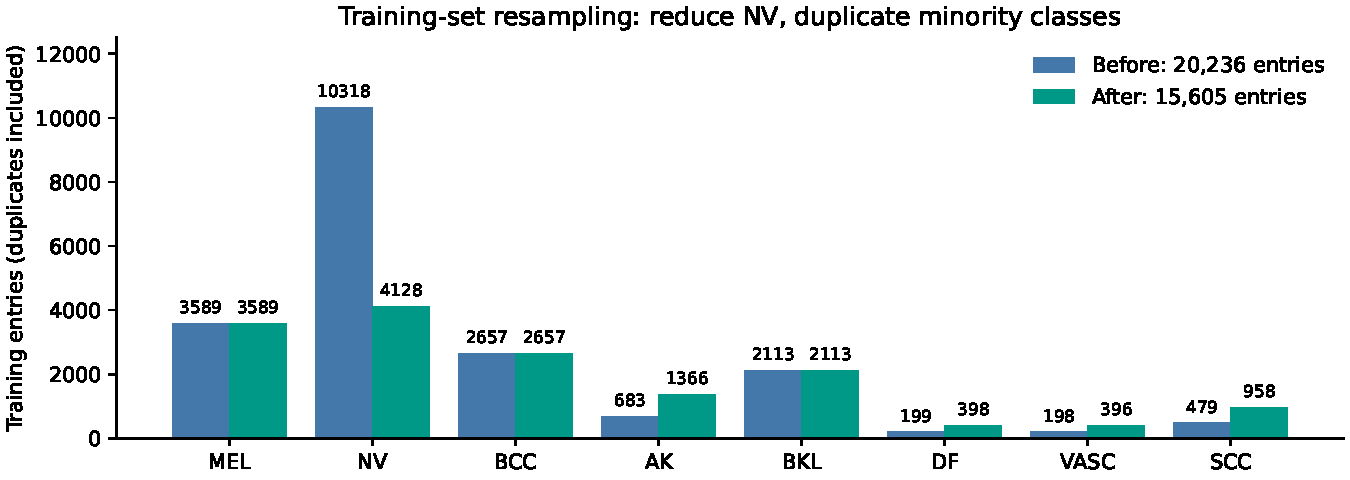
\includegraphics[width=0.92\linewidth,height=3.6cm,keepaspectratio]{../evidence/resampling_before_after.pdf}
\end{center}
\vspace{-1em}
{\footnotesize\textbf{Training distribution before/after resampling.} Counts are row sums of archived training confusion matrices for focal runs without/with resampling, on the same 80\% training-group split. These are training entries, including duplicates, rather than full-dataset counts.}

\newpage
\section{Minimal federated setup}
The launcher starts one Flower SuperLink and four SuperNodes on the same machine. These nodes represent simulated hospitals rather than verified institutional cohorts. They share access to the local dataset, while application code selects disjoint partitions for each client. A globally initialized ResNet-18 is sent to all participating hospitals. Each trains for two local epochs and returns weights and scalar metrics; no raw image arrays are included in these training replies.

\textbf{Partitioning.} The saved experiment uses a Dirichlet partition with concentration $\alpha=0.5$ and seed 42. Per-class client shares are drawn once and applied to training and validation groups. Whole lesion groups are assigned to clients; the same target class proportions are used for training and validation, with integer/group-size effects. This simulates label skew, not scanner or hospital-specific covariate shifts.

\textbf{Aggregation.} The run performs ten FedAvg rounds with all clients selected for training and validation. If hospital $k$ has $n_k$ training examples, its local model contributes as
\[
w^{(t+1)}=\sum_{k=1}^{4}\frac{n_k}{\sum_j n_j}\,w_k^{(t+1)}.
\]
The optimizer is recreated at each local training call. Centralized early stopping and learning-rate scheduling are not used by this federated local loop. FedProx is available in the implementation, but the archived run has $\mu=0$ and is FedAvg.

The saved run configuration records training/validation/test group fractions 0.3/0.1/0.1, batch size 32, learning rate $10^{-4}$, and two loader workers. Across clients there are 7,539 training and 2,667 validation images. The test split is reserved but is not evaluated in the saved federated workflow. \textbf{Configuration reconstruction.} The archived baseline histories and federated source support a working reconstruction using AdamW, weight decay $10^{-3}$, focal loss ($\gamma=2$), and the baseline transformations. Final-model validation replay supports focal loss and the validation pipeline; optimizer and training-only augmentations remain inferred. The federated data path does not apply resampling. Evidence and confidence labels are preserved separately. The smaller training fraction and batch size define a distinct exploratory experiment, motivating further matched runs.

\begin{center}
\small
\begin{tabular}{lrrrr}
\toprule
Hospital & Training images & Validation images & Round-10 val. accuracy & Round-10 val. macro-F1\\
\midrule
0 & 765 & 297 & 0.4411 & 0.2651\\
1 & 1,588 & 538 & 0.4312 & 0.2905\\
2 & 2,813 & 958 & 0.8653 & 0.3846\\
3 & 2,373 & 874 & 0.6865 & 0.4478\\
\bottomrule
\end{tabular}
\end{center}

\textbf{Metric interpretation.} The server averages client metrics using the corresponding split's sample counts. Its macro-F1 is therefore $\sum_k(n_k/N)\,\mathrm{F1}_{\mathrm{macro},k}$, not macro-F1 computed from pooled predictions. Missing local classes receive zero F1, further affecting comparability. Validation evaluates the aggregated global model; training metrics describe local models during their last local epoch, not the final global model evaluated on pooled training data.

The final aggregate validation accuracy is 0.6719 and weighted client macro-F1 is 0.3730. The maximum validation macro-F1 is 0.3837 at round 9; the saved weights are from round 10, rather than a validation-selected best checkpoint. Per-hospital validation macro-F1 ranges from 0.2651 to 0.4478. Federated results are saved as JSON, plots, and final weights in a timestamped output directory; this workflow does not log to MLflow.

\newpage
\section{Preliminary analysis and trustworthiness directions}
\begin{center}
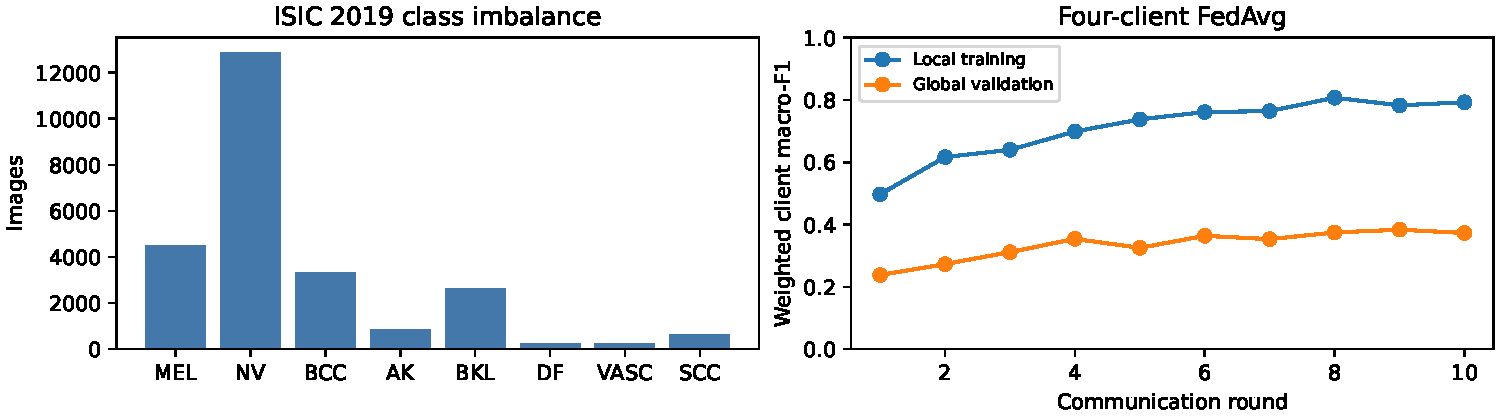
\includegraphics[width=\linewidth]{../evidence/overview.pdf}
\end{center}
\vspace{-1em}
\textbf{Figure 1.} Left: full-dataset counts from the archived EDA CSV, rather than its historical split counts. Right: archived federated macro-F1 curves. The widening gap concerns local-training versus global-validation measurements and is consistent with limited generalization, but does not isolate a causal mechanism.

\textbf{Centralized findings.} AdamW fine-tuning at $10^{-4}$ yields stronger observed validation macro-F1 than the interrupted SGD and AdamW-at-$10^{-2}$ trials. Those trials differ in training duration and are not a controlled optimizer benchmark. At their minimum-validation-loss checkpoints, validation macro-F1 is 0.5319 for cross entropy, 0.5327 for focal loss, and 0.5382 for focal loss with resampling. The last result does not translate into higher held-out test macro-F1. For the focal model without resampling, test recall is 0.9060 for NV and 0.2222 for DF, illustrating why aggregate accuracy can conceal weak minority-class performance.

\textbf{Centralized versus federated.} The focal centralized checkpoint has validation accuracy 0.7338 and macro-F1 0.5327; final FedAvg validation accuracy is 0.6719 and weighted client macro-F1 is 0.3730. These are descriptive observations, not a controlled performance ranking: training fractions, batch sizes, optimization schedules, and F1 aggregation differ; some federated training settings are reconstructed rather than directly recorded. Centralized test scores must not be treated as equivalent to federated validation scores. A matched experiment should use the same training pool, validation/test definitions, initialization, preprocessing, and budget, then sum client confusion matrices to compute pooled macro-F1 without sharing raw images.

\textbf{Stage 2 directions.} (1) Measure worst-client and minority-class recall alongside mean performance, including support counts and uncertainty. (2) Repeat matched centralized/FedAvg runs across seeds and Dirichlet concentrations to study robustness to label skew; evaluate FedProx as a separate extension. (3) Assess calibration and clinically meaningful error patterns before considering deployment. (4) Evaluate explicit privacy mechanisms if privacy is selected: exchanging model updates alone is not a privacy guarantee. The simulation provides neither secure aggregation nor differential privacy evidence, and does not demonstrate patient-level separation.

{\small
\begin{thebibliography}{3}
\bibitem{ahmad2026}
I. Ahmad, M. Khubaib, and S. M. Altowaijri.
Benchmarking Class Imbalance Mitigation Strategies Across Deep CNN Architectures for Skin Cancer Classification.
\emph{Diagnostics}, 16(16):2571, 2026.
\href{https://doi.org/10.3390/diagnostics16162571}{doi:10.3390/diagnostics16162571}.

\bibitem{gayatri2024}
E. Gayatri and S. L. Aarthy.
Reduction of overfitting on the highly imbalanced ISIC-2019 skin dataset using deep learning frameworks.
\emph{Journal of X-Ray Science and Technology}, 32(1):53--68, 2024.
\href{https://doi.org/10.3233/XST-230204}{doi:10.3233/XST-230204}.

\bibitem{cino2025}
L. Cino, C. Distante, A. Martella, and P. L. Mazzeo.
Skin Lesion Classification Through Test Time Augmentation and Explainable Artificial Intelligence.
\emph{Journal of Imaging}, 11(1):15, 9 January 2025.
\href{https://doi.org/10.3390/jimaging11010015}{doi:10.3390/jimaging11010015}.
PMID: 39852328; PMCID: PMC11766406.

\end{thebibliography}
}
\end{document}
